\documentclass{article}
\usepackage{neurips_data_2021}
\usepackage[utf8]{inputenc}
\usepackage{booktabs}
\usepackage{hyperref}
\usepackage[capitalize]{cleveref}
\usepackage{graphicx}
\usepackage{color}
\newcommand{\tbo}{}
\title{The CPD Data Set: Officers, Complaints, and Tactical Response Reports from the Chicago Police Dept}

\begin{document}


\maketitle

\begin{abstract}
	We present a new dataset focusing on the personnel and activities of the
	Chicago Police Department (CPD). The data was curated starting multiple
	data releases by the Chicago Police Department following a series of
	requests under the the Freedom of Information Act. In this document we give
	a detailed description of the content of the dataset as well as the data
	cleaning process.
\end{abstract}

\section{Introduction}

There has been some ML work done on individual correlates that are associated
with (and potentially predictive of) police misconduct. Scholars have looked at
the association between misconduct and an individual officer's race, gender,
years on the force, prior instances of misconduct, stages of officer career,
assigned unit. But research suggests that violence emerges not just at the
individual level but also at the population level from the interaction of
individuals in groups—think of gangs. 

 
We offer a dataset that allows ML to investigate the influence of police social
networks on police misconduct. The dataset allows ML to explore features of
police social networks that might be associated with and potentially predictive
of adverse police encounters with civilians or other misconduct. These network
correlates can include the architecture and structures of social networks in
departments and smaller subunits within a department—for example, the number of
connections each officer has, the strength of those connections, the bridge
positions that some officers have across subunits. More innovatively, ML can be
used in the way it is often used to study disease dynamics: ML can find the
patterns of behavior (clustering, outbreaks, spreading, geographic hotspots) on
a network that might be associated with violence. 

 
We show how to use complaint datasets from a police department in a major city
to investigate the influence of social networks on police misconduct and
violence. 


The original data was obtained following a series of requests covered by the
Freedom of Information Act (FOIA) to the Chicago Police Department (CPD) and
the Civilian Office of Police Accountability (COPA). The information which was
requested pertained to CPD's personnel and its activities.

\textbf{TODO:} ideally say a bit more about the history of these FOIA requests.
Apparently they were initiated by individual journalists and lawyers and were
later coordinated by the Invisible Institute which ultimately became the
central location were (almost) all the data is currently available.

\begin{table}[h]
	\begin{center}
\begin{tabular}{@{}llll@{}}
	\toprule
	request \#&received&requested&description\\
\midrule
	\texttt{P0-58155}&2017-04-17& &Officer roster\\
	\texttt{P4-41436}&2018-03-21& &Officer roster\\
		\texttt{P0-52262}&2016-12-04&2016-09-19&Unit assignment\\
		\texttt{16-1105}&2016-03-11&2016-02-10&Unit assignment\\
	\texttt{P0-46957}&2016-06-29&2016-04-22&Complaints (CPD)\\
	\texttt{18-060-425}&2018-08-28&2018-08-20&Complaints (COPA)\\
	\texttt{P0-46360}& & &Tactical Response Reports\\
\bottomrule
\end{tabular}
\caption{Summary of the FOIA requests to the CPD and COPA contained in our repository.}
\label{table:summary}
\end{center}
\end{table}

Each FOIA request is identified by a request number, \cref{table:summary} gives
an overview of all the requests made to the CPD and COPA that are present in
our repository. This information is also available in the file
\texttt{dataset.csv} in the root folder of the repository. The original
data—that is the files received after each FOIA request—are present in the
\texttt{raw/} folder of the repository, with one subfolder for each request,
identified by the request number. When available, each subfolder also contains
the formal request letter as well as the reply letter from the CPD or COPA,
which are useful in understanding what data was included in each dataset.
Some additional comments about the data:
\begin{itemize}
	\item \emph{Officer roster:} lists all officers (past or present) employed
		by the CPD along with attributes such as year of birth, age, race,
		gender, appointment date, resignation date, etc.
	\item \emph{Unit assignment:} the CPD is organized into (500 or so?) units.
		Each officer can be assigned to one or multiple units and these
		assignments can change over time. The unit assignment datasets contain
		one record for each officer and each unit they were assigned to, with
		the start date and end date of this assignment.
	\item \emph{Complaints:} formal complaints filed by citizens against police
		officers. Complaints are identified by a complaint number, and there is
		one record for each complaint and each officer listed on the complaint,
		indicating the allegation made against them, result of the
		investigation of the allegation (with possible sanction), etc.
	\item \emph{Tactical Response Reports:} these are forms that officers are
		required to file after each incident for which the officer's response
		involved use of force.
\end{itemize}

Let us already mention an inherent difficulty in making use of this data, which
will be discussed in \cref{sec:linking}: there is no number/identifier which
uniquely identifies officers across datasets. Such an identifier probably
exists internally in the CPD, but was never included in the data released to
the public. One would be tempted to believe that the \emph{badge number} (also
sometimes referred to as \emph{star number} of an officer is such an
identifier, but unfortunately, it changes over the course of an officer's
career in the CPD, and a given badge number can be reassigned to different
officers when they are no longer in use.


\subsection{Related Work}

Police records datasets

This data was originally obtained by the Invisible Institute and has been publicly available for about 3 years here \url{https://github.com/invinst/chicago-police-data}
(limitations: not well organized or reproducible, problematic/incorrect linkage, missing unit information, units are not semantically grouped)

Gang violence data



\section{The CPD Data} \label{sec:data}
The original raw data released by the CPD, 
the code to generate the cleaned data, and the source code for this document 
are available at \url{https://github.com/chicago-police-violence/data}.
The data processing code is written in Python, and the documentation is written in \LaTeX.
\texttt{Make} is used to coordinate the various processing steps and easily reproduce them.
Refer to \url{README.md} in the repository for details regarding system requirements and 
how to generate the cleaned data.

\subsection{The raw data: origin, description, and challenges}
The first raw data files in this repository were obtained by J.~Kalven, an 
independent journalist, who filed Illinois Freedom of Information Act requests with 
the Chicago Police Department regarding complaints filed against officers. 
In Kalven v.~City of Chicago \cite{kalven2014}, an Illinois appellate court issued
a general ruling that documents bearing on allegations of
police abuse are public information. Following 
the decision, the non-profit
Invisible Institute began to collaborate with Kalven 
and the University of Chicago's Mandel Legal Aid
Clinic to follow up on earlier FOIA requests and to file new ones. The data
disclosed in response to these earlier and now ongoing FOIA requests were made available
online as part of the Citizens Police Data Project \cite{cpdp}.
These data form the basis of the cleaned and linked data set provided by the present work.

\begin{table}[h]
	\begin{center}
\begin{tabular}{@{}lllll@{}}
	\toprule
	request \#&received&requested&description\\
\midrule
	\texttt{P0-58155}&2017-04-17& &Officer roster\\
	\texttt{P4-41436}&2018-03-21& &Officer roster\\
	\texttt{P0-52262}&2016-12-04&2016-09-19&Unit assignments\\
	\texttt{16-1105}&2016-03-11&2016-02-10&Unit assignments\\
	\texttt{P0-46957}&2016-06-29&2016-04-22&Complaints (CPD)\\
	\texttt{18-060-425}&2018-08-28&2018-08-20&Complaints (COPA)\\
	\texttt{P0-46360}& & &Tactical Response Reports\\
	\texttt{P0-46987}&2016-05-13&2016-04-25&Unit names\\
	\texttt{P0-61715}& &2017-07-26&Awards\\
	\texttt{P5-06887}&2019-10-11&2019-07-19&Awards\\
	&2017-09-27&2017-09-13&Salary\\
\bottomrule
\end{tabular}
\caption{Summary of the FOIA requests contained in our repository (blanks are missing entries).}
\label{table:summary}
\end{center}
\end{table}

The raw data files are contained in the \url{raw/} folder of the
repository. Each subfolder corresponds to a FOIA request, which is
generally identified by a request number. \cref{table:summary} gives
an overview of all the requests that we include in
our repository; this meta-information is also included in the \url{raw/datasets.csv}
file in the repository. The subfolders contain the data provided by the city
in response to their corresponding FOIA requests, which typically comprises multiple
Excel spreadsheets. In addition, when available, the subfolders contain formal correspondence 
regarding the request, which often provides useful contextual information in understanding the data.  

In particular, the raw data files contained in the repository
provide the following information: {\color{red} todo: year ranges for each?}
\begin{description}
	\item[Officer roster:] a list of all officers (past and present) employed
		by the CPD along with attributes such as year of birth, age, race,
		gender, appointment date, resignation date, etc.
	\item[Unit assignments:] the CPD is organized into over 200 units.
		Each officer can be assigned to one or multiple units and these
		assignments can change over time. The unit assignment datasets contain
		one record for each officer and each unit they were assigned to, with
		the start date and end date of this assignment.
	\item[Complaints:] formal complaints against police officers, filed both by citizens
                and internally within the department. Complaints are identified by a complaint number. 
                There is one record for each complaint and each officer listed on the complaint,
		indicating the allegation made against them, result of the
		investigation of the allegation (with possible sanction), etc.
	\item[Tactical Response Reports:] these are forms that officers are
		required to file after each incident for which the officer's response
		involved use of force. Each record contains... {\color{red} thibaut fill in, similar to above for complaints}
        \item[Unit names:] the (human-readable) name of each (past and present) unit in the CPD. 
                Unit names also appear occasionally where unit numbers are listed in the other data files.
        \item[Awards:] a list of all awards requested for officers in the CPD, including 
                award tracking number, reference number, award type, request date, requester name,
                etc.
        \item[Salary:] a list of officers from 2002--2017 including their salary, position, and pay grade.
\end{description}

Challenges:
- time varying attributes: badge numbers (stars), unit numbers, job titles change over time. but 
more unusual things change too -- names (e.g.~marrying), appointment dates (e.g.~when db entries are corrected)
- systematic errors: unit history backwards, 
- multiple DBs: salary comes from different DB from the rest of it. names were entered differently, etc.
- ambiguous field meanings: salary has 2 different dates for apt, etc.
- dead entries: 
- inconsistent entries across different files: officers missing from history, roster, present in salary, etc
- idiosyncratic errors: 


\subsection{Initial Cleaning}

The files initially released by the CPD as a reply to the FOIA requests are for
the most part Excel spreadsheets, with inconsistent formatting and which can
thus be difficult to process programmatically. As an example, the reader is
invited to open the file
\texttt{p046957\_-\_report\_1.1\_-\_all\_complaints\_in\_time\_frame.xls}
available in the folder \texttt{raw/P0-46957/}. As can be seen, each record in
this file is spread over two rows of the spreadsheet, with the field names
repeated at the beginning of the second row for each record.

The goal of the cleaning step is thus to produce ``reasonable'' CSV files from
the original files, with the minimum requirement that each record be presented
on a single line after this step. The code for this cleaning step is contained
in the files \texttt{datasets.py}, \texttt{parse.py} and
\texttt{parse\_p046957.py} in the \texttt{src/} folder and the entire step can
be applied by running \texttt{make parse} in the root of the repository. This
creates the folder \texttt{parsed/} containing the clean CSV files.

As can be seen by inspecting the code, the decisions made at this stage are, we
believe, uncontroversial as they only consists of:
\begin{itemize}
	\item unifying field names across datasets, so that the same type of data
		is always identified in the saw way (for example, \texttt{Appointment
		Date}, \texttt{Appt Date}, \texttt{appointment\_date} are all mapped to
		\texttt{appointment\_date}.
	\item unifying field values across datasets. For example, the gender of an
		officer is indicated as a single letter \texttt{M} or \texttt{F} in
		some datasets or as \texttt{Male}, \texttt{Female} (based on the data
		release, it does not seem that the system used by the CPD has an option
		to represent non-binary officers).
	\item parsing values into the correct data type or format. For example,
		dates are formatted differently depending on the dataset, and we map
		everything to the ISO 8601 format.
\end{itemize}

Consequently, for someone planning to use the data in the present repository,
there is virtually no reason not to start at the minimum from the output of
this cleaning step. The subsequent steps required making more difficult and
debatable decisions, so depending on the application, researchers might want to
perform them differently, but in all cases, those alternative decisions can
branch off from the output of the cleaning step.

\subsection{Linking and Merging Datasets}\label{sec:linking}

\subsubsection{Officer matching}

As already alluded to, the main challenge at this step is that there is no
identifier uniquely identifying officers across records. In other words, there
is no foolproof way to know if two different records correspond to the same
officer, \emph{even within the same dataset} (for example the same officer
could appear with slightly different attributes on two different complaint
records).

We thus need to design a matching method striking a balance between
\begin{itemize}
	\item being loose enough to avoid type II error (false negatives). If the
		same officer appears with slightly different attributes across two
		records, we do not want our matching method to believe it is two
		different officers.
	\item being strict enough to avoid type I error (false positives). We do
		not want to merge two different officers into a single identity.
\end{itemize}

The difficulty in achieving this balance is that perhaps surprisingly
\emph{none of the attributes of a given police officer are guaranteed to be
stable over time}. Most notably, officers' names change over time, for example
to fix data entry errors or in case of legal name changes. However, we observed
two attributes, present in almost all original datasets and which seem
remarkably stable over the time: \emph{appointment date} and \emph{birthyear}.
These two attributes thus proved very valuable to disambiguate officers with
identical names.

In order to match officers across two datasets, we developed an \emph{iterative
pairwise matching procedure} that makes iterative passes over the datasets.
During each pass, a subset of the officer attributes present in both datasets
is selected as the matching criterion, and a pair of officers (one from each
dataset) is identified as a \emph{match} if (i) their attributes from the
chosen subset match, and (ii) if they are the only two officers matching on
these attributes. Once a pair is identified as a match, it is put aside, and
the next pass is performed on the remaining unmatched officers. After all the
passes are done the leftover officers are declared as different officers. By
constructing a hash table mapping a subset of attributes to the list of
officers sharing these attributes, each pass can be performed in linear time,
so the overall running time of the procedure is $O\big(P(N_1+N_2)\big)$ where
$P$ is the number of passes and $N_1, N_2$ are the number of officers in each
dataset.

To fully specify the matching procedure we thus need to specify which subset of
attributes is chosen as the matching criterion at each pass. For this, we go
from the stricter to the looser criterion: for the first pass, we choose
a subset \emph{all} the attributes which are present in two datasets, and then
start removing attributes one by one. For example, one can remove the
\emph{last name} attribute for the second pass to match a pair of officers
whose last names are different but match on all the remaining attributes, thus
identifying an officer whose last name changed between the releases of the two
datasets. The advantage of going from stricter to looser is two fold:
\begin{itemize}
	\item starting from the strictest set of attributes identifies the
		\emph{unambiguously matching pairs}, that is, the ones which are
		a clear match and which, thankfully, constitute the vast majority of
		officers (typically around 80-90\% of officers are matched during the
		first pass \textbf{TODO check}). Since the next passes will only be
		performed on the remaining unmatched officers, this removes a lot of
		potential ambiguities which could occur once the set of attributes is
		reduced.
	\item since the vast majority of officers is matched during the first pass,
		it becomes feasible during the subsequent passes to visually inspect all
		the matched pairs and assess whether the chosen set of attributes was
		too strict or too lose (\textbf{TODO:} explain how to activate
		debugging information in the code).
\end{itemize}

We note that there is still some amount of subjective judgment involved,
following a visual inspection of the second and subsequent passes, to decide
which sets attributes are ``acceptable'' (that is, for which the probability of
two persons sharing these attributes in a population of the size of the CPD is
extremely small). This is also how we decide that sufficiently many passes have
been performed: when it would seem likely to introduce a type I error by
matching any of the remaining officers. As a general rule of thumb we erred on
the side of favoring type II errors over type I errors. That is, we only
matched officers when it would seem extremely unlikely that they correspond to
two different individuals).

\textbf{TODO:} table of officer attributes in each dataset

\textbf{TODO:} explain the few subtleties where we don't use equality to match
attributes (for example when matching age and birthyear, where the age only
lets us identify the birthyear with an accuracy of 1 year). Or with stars,
where we test whether a star number is contained in the subset of known stars
for this officer.

With this procedure at hand we can thus link officers across datasets starting
from the most similar datasets first (for which we expect to have the least
amount of ambiguity). That is we first link \texttt{P0-58155} to
\texttt{P4-41436}, then \texttt{P0-52262} to \texttt{16-1105} and then the
remaining datasets \textbf{expand}

\textbf{TODO} give in appendix table summarizing which subset of attributes are
used at each linking operation 

\subsubsection{Roster consolidation}

A byproduct of matching officers across datasets is that for each officer, we
now have as many “profiles” as the number of datasets in which they appear,
where by \emph{profile} we mean a collection of attributes. Note that each
profile can contain a different subset of attributes (since not all attributes
are present in each dataset) and that a given attribute might take a different
value in different profiles of the same officer (since the iterative matching
procedure is not restricted to performing strict matching).

We are thus faced with the task of “consolidating” the different profiles of
a given officer into a single profile. Of course, if an attribute is present in
a single profile, and absent from the others, this is the value we keep in the
consolidated profile. But if an attribute appears with different values across
different profiles, we choose the value coming from the profile corresponding
to the \emph{most recent data release}.

\subsubsection{Unit assignment history} TODO.


\subsection{Unit identification and binning}


% !TEX root = ../main.tex

\section{Exploratory Analysis and Examples} \label{sec:analysis}

In this section, we provide examples and use-cases on the dataset. Code to
reproduce our examples is available online, in the \texttt{examples} folder.

\subsection{Visualizations}

\paragraph{Roster.}
%The file \texttt{roster.csv} contains information about $N=35{,}430$ CPD
%officers. For each officer --- identified by a Unique Identifier (``uid''),
%\texttt{roster.csv} provides, among other covariates, the officer's name,
%gender, race, birthyear, appointment and resignation dates. It is
%straightforward  to use the data to generate summary statistics, e.g., using
%appointment and resignation dates to understand the number of appointments,
%retirements as well as active officers over the years of  (\Cref{fig:history}).
%We report in \Cref{tab:stats} some 


\begin{figure}[t!] 
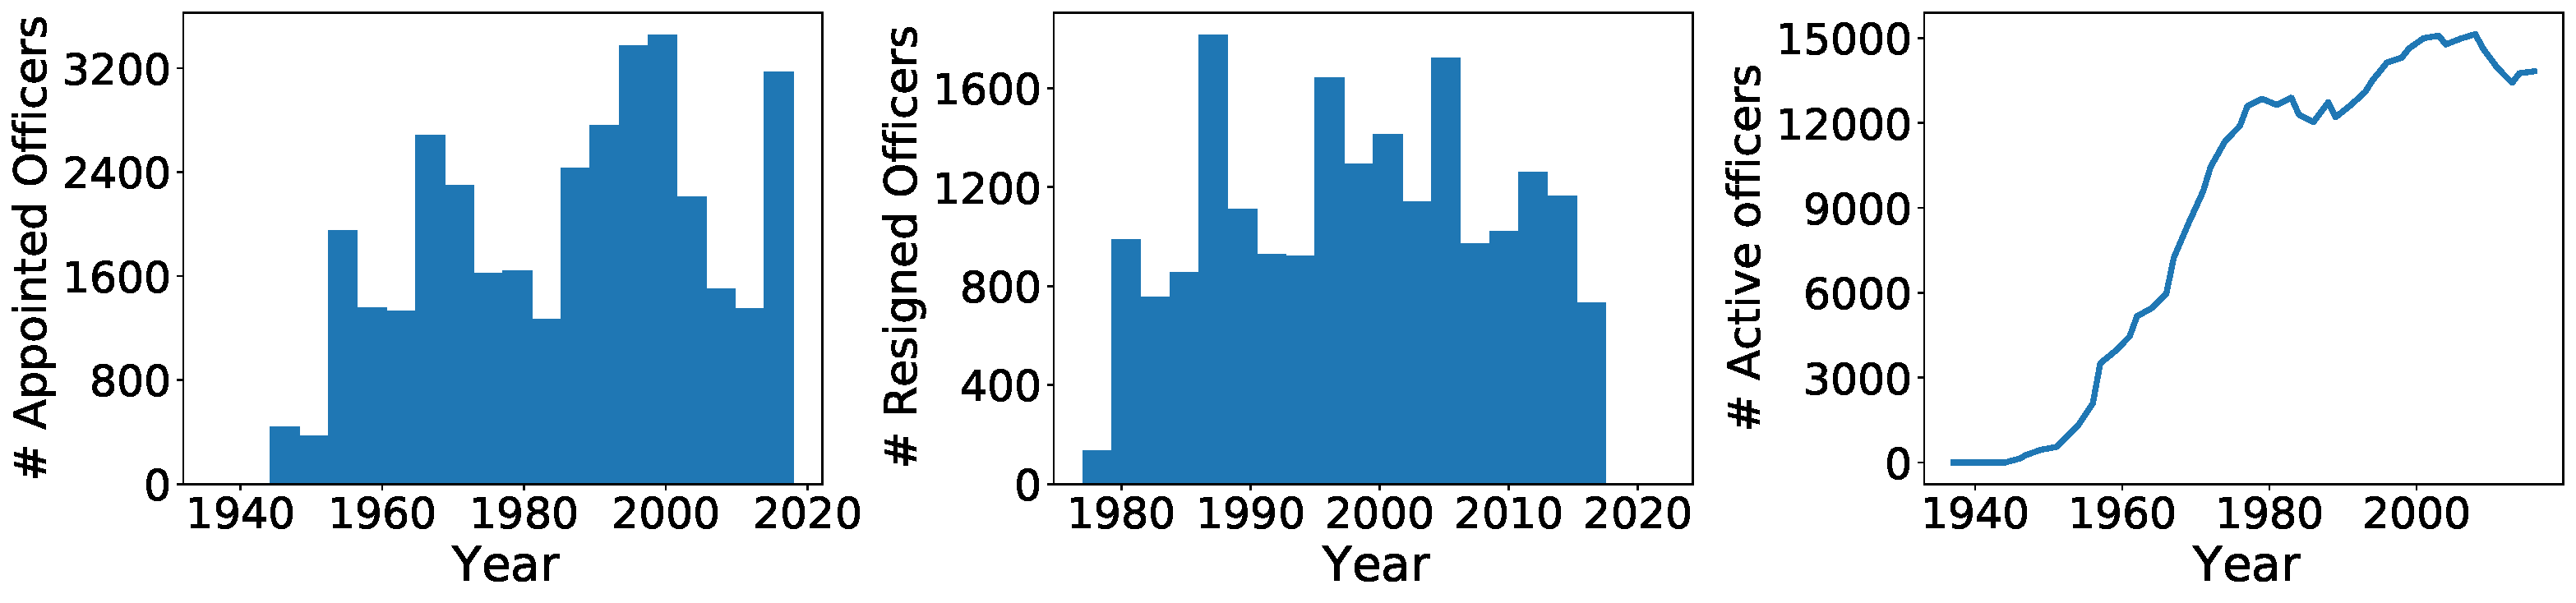
\includegraphics[width=\textwidth]{figs/history} 
\caption{Appointments (left), resignations (center), and the number of active
officers (right) appearing in the CPD roster database from the years 1940 to 2019.}
\label{fig:history}
\end{figure}

\begin{table}[t!]
\caption{Counts of officers (first row) and active officers (resignation date not before 2019-01-01, second row). 
Note that ``race'' and ``gender'' are per the CPD's coarse categorizations.} \label{tab:stats}
\begin{tabular}{l|c|c|c|c|c|c|c|c|c|}
\cline{2-3} \cline{5-10}
                                               & \multicolumn{2}{c|}{\textbf{Gender}} & \multicolumn{1}{l|}{} & \multicolumn{6}{c|}{\textbf{CPD Race Category}}                                                                                                                                                   \\ \cline{2-3} \cline{5-10} 
                                               & {\textbf{M}}   & {\textbf{F}}   &                       & {\textbf{White}} & {\textbf{Black}} & \multicolumn{1}{l|}{{\textbf{Hisp.}}} & {\textbf{Asian/P.I.}} & \multicolumn{1}{l|}{{\textbf{Indig.}}} & {\textbf{Bl. Hisp.}} \\ \cline{1-3} \cline{5-10} 
\multicolumn{1}{|c|}{\textbf{All}}    & 28316                 & 7122                  &                       & 21047                   & 8599                    & 4811                                         & 582                     & 67                                              & 9                           \\ \cline{1-3} \cline{5-10} 
\multicolumn{1}{|c|}{\textbf{Active}} & 11118                 & 4452                  &                       & 7241                    & 3895                    & 3596                                         & 467                     & 40                                              & 9                           \\ \cline{1-3} \cline{5-10} 
\end{tabular} 
\end{table}

\begin{figure}[h] 
	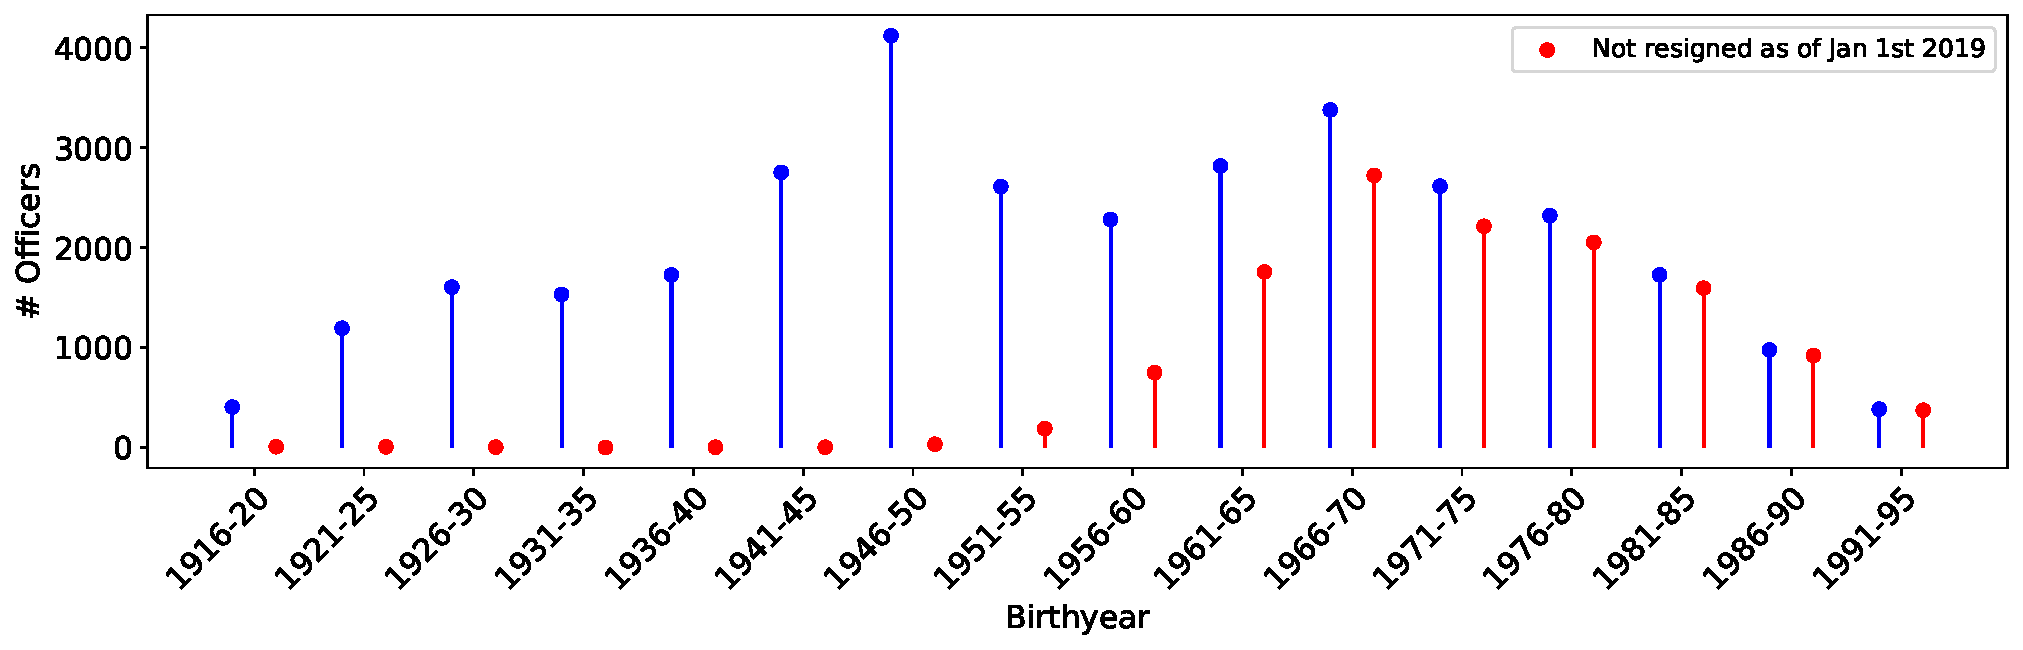
\includegraphics[width=\textwidth]{figs/history_by} 
	\caption{Historical data from the CPD. Birthyears for officers in the CPD dataset: blue dots count all officers, while red count only officers who are ``active'' as of January 1st, 2019.} \label{fig:history_by}
\end{figure}

We use the file \texttt{roster.csv} to obtain basic statistics about officers in the CPD dataset. The data contains informations about officers whose appointment dates back to 1936, all the way to 2018 (see \Cref{fig:history}). An important remark to be made is that the data becomes sparser, and less reliable in earlier years. For example, we report in the right subplot of \Cref{fig:history} the number of active officers (vertical axis) as a function of time (horizontal axis): we notice that this number increases sharply between 1940 and 1980. This should be interpreted as a consequence of the lack of data availability for those early years. We also report summary statistics on gender and the CPD race category in \Cref{tab:stats}, and information about officers' birthyears in \Cref{fig:history_by}.

\paragraph{Units.} 
\begin{figure}[h] 
	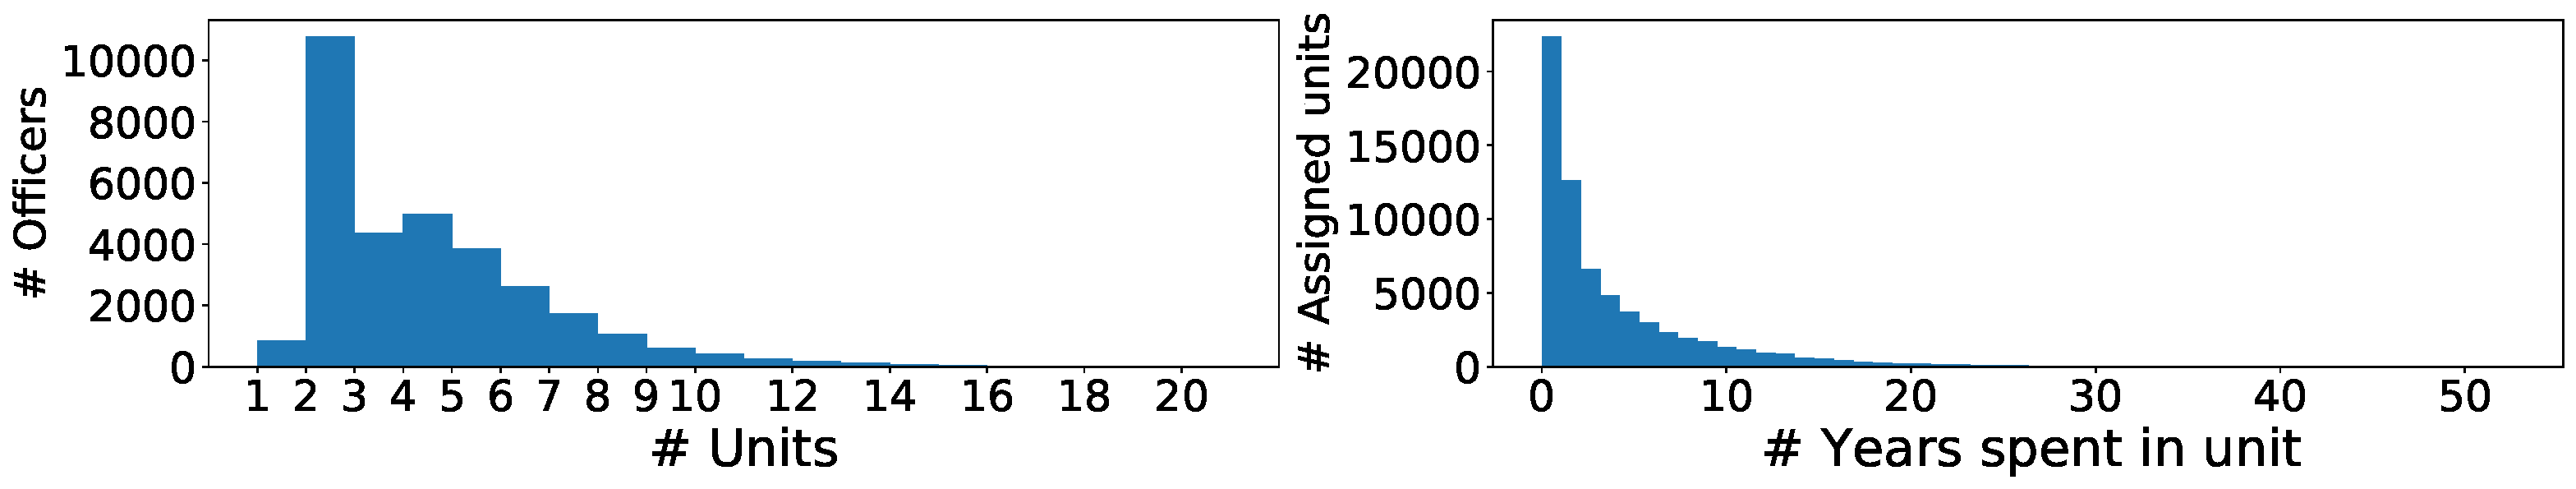
\includegraphics[width=\textwidth]{figs/units_officers} 
	\caption{Units assignments. Left: number of units assignments for officers in the CPD over the course of their career. Right: histogram for the number of years spent in each unit for ``completed'' units assignments only --- that is, assignments that had terminated at the time of data-collection.} \label{fig:units}
\end{figure}


We report summary statistics about the number of units an officer is assigned to, and the duration of such appointments in \Cref{fig:units}. The modal number of units appointments is 2: officers typically first joins the acadamy (unit 44), for one or two years, before moving on to a different, often terminal, unit. 
 
\paragraph{Complaints.} 
\begin{figure}[h] 
	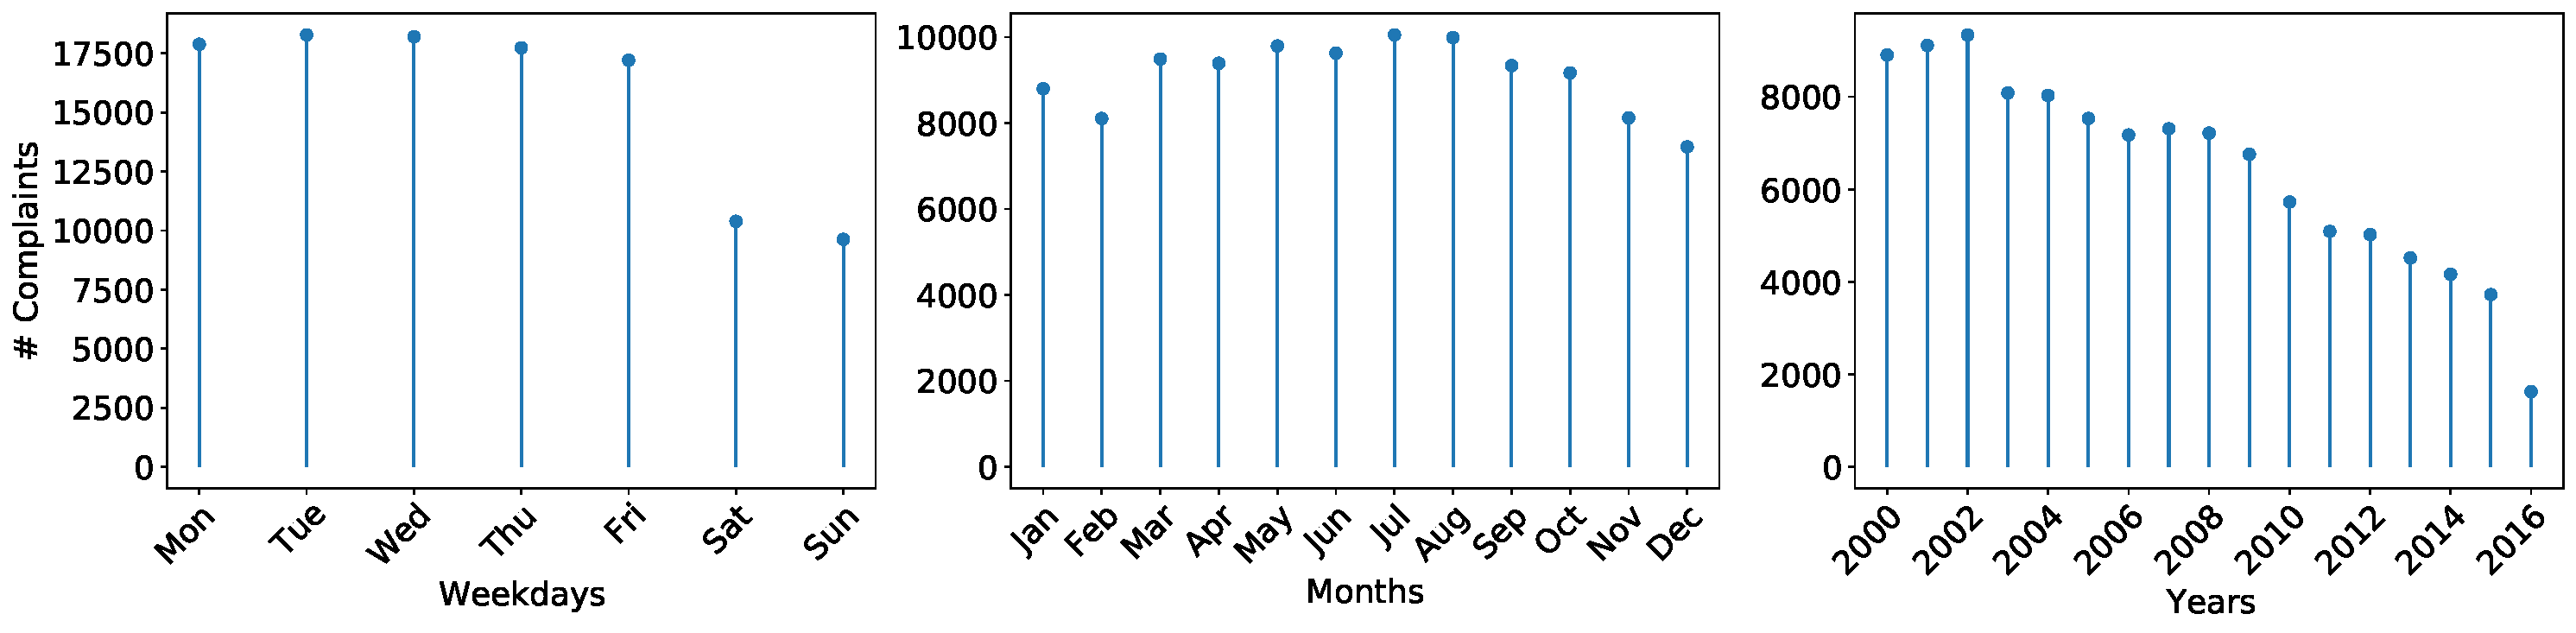
\includegraphics[width=\textwidth]{figs/complaints_times} 
	\caption{Temporal data for complaints.} \label{fig:complaints_times}
\end{figure}
\begin{figure}[h] 
	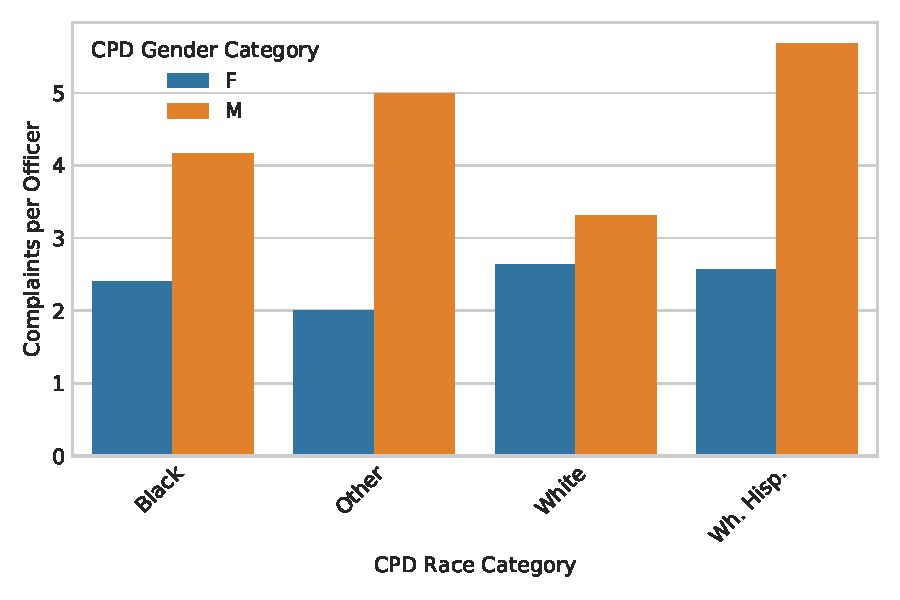
\includegraphics[width=\textwidth]{figs/complaints} 
	\caption{Temporal data for complaints.} \label{fig:complaints}
\end{figure}

We report in \Cref{fig:complaints} temporal information about complaints filed against the CPD. Interestingly, fewer complaints get filed during the weekends (although, the number of TRRs is higher then --- see \Cref{fig:trrs_times}). Moreover, complaints tend to be higher in the warmer months. Last, we notice that the number of complaints filed kept reducing over the years --- potentially as a consequence of the perception of ineffectiveness of such complaints.

\paragraph{Tactical Response Reports.}

\begin{figure}[h] 
	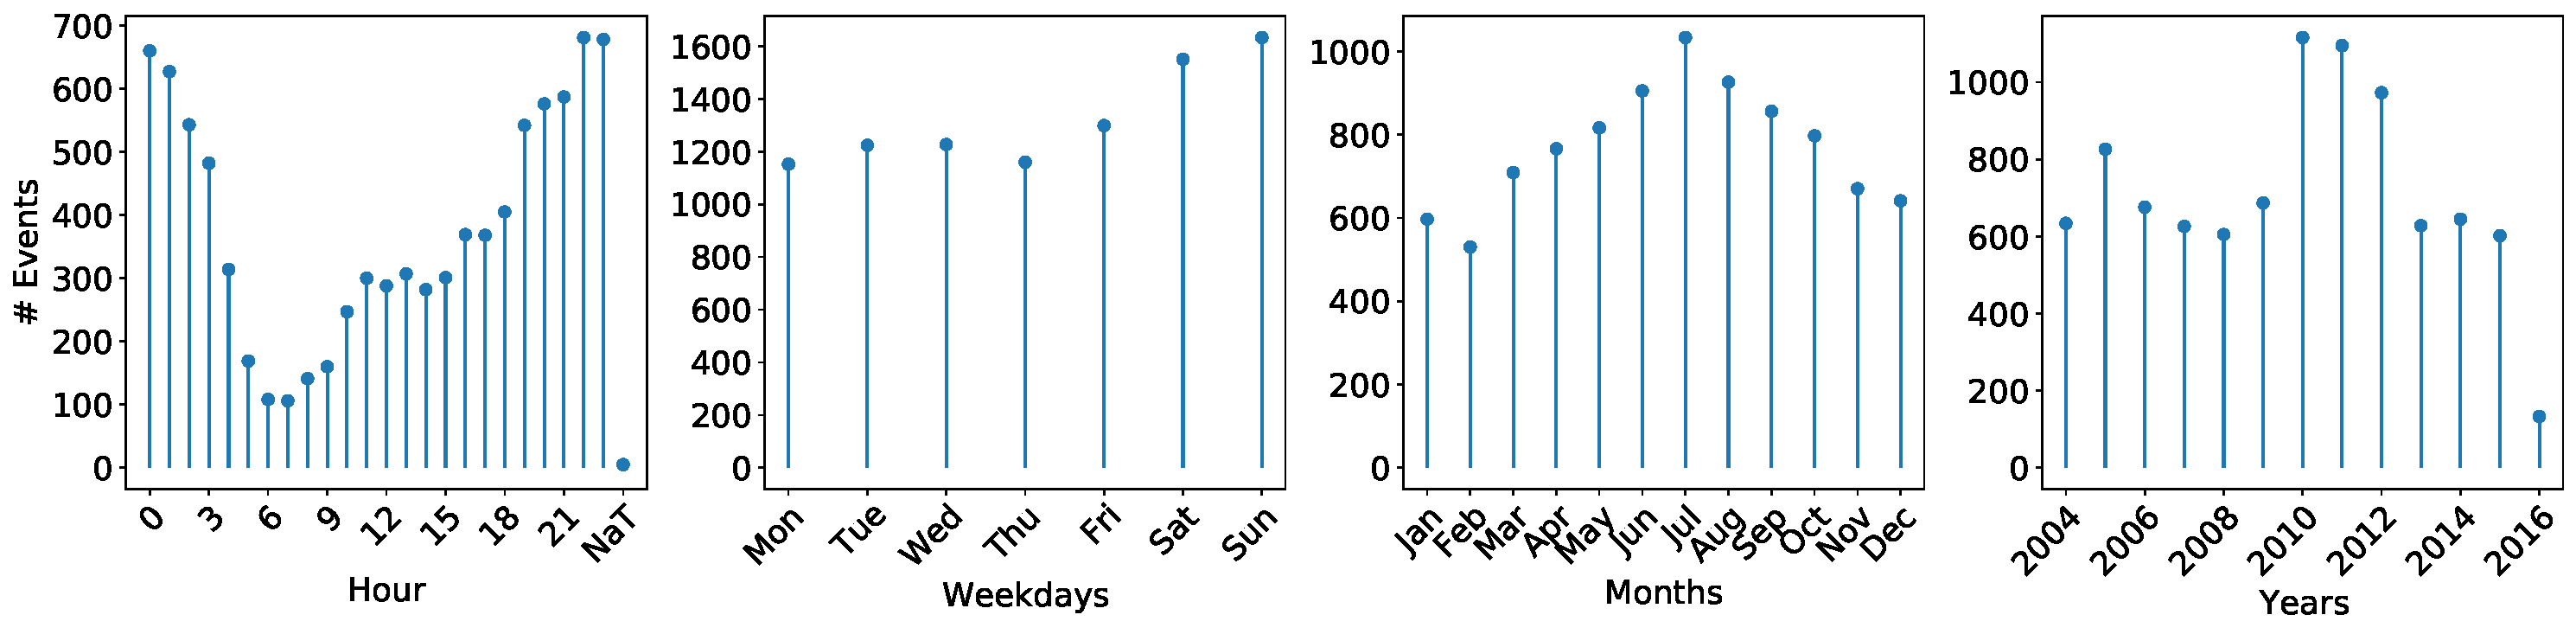
\includegraphics[width=\textwidth]{figs/trrs_times} 
	\caption{Temporal data for TRRs. Left: time during the day; mid-left: time during the week; mid-right: month; right: year.} \label{fig:trrs_times}
\end{figure}

\begin{figure}[h] 
	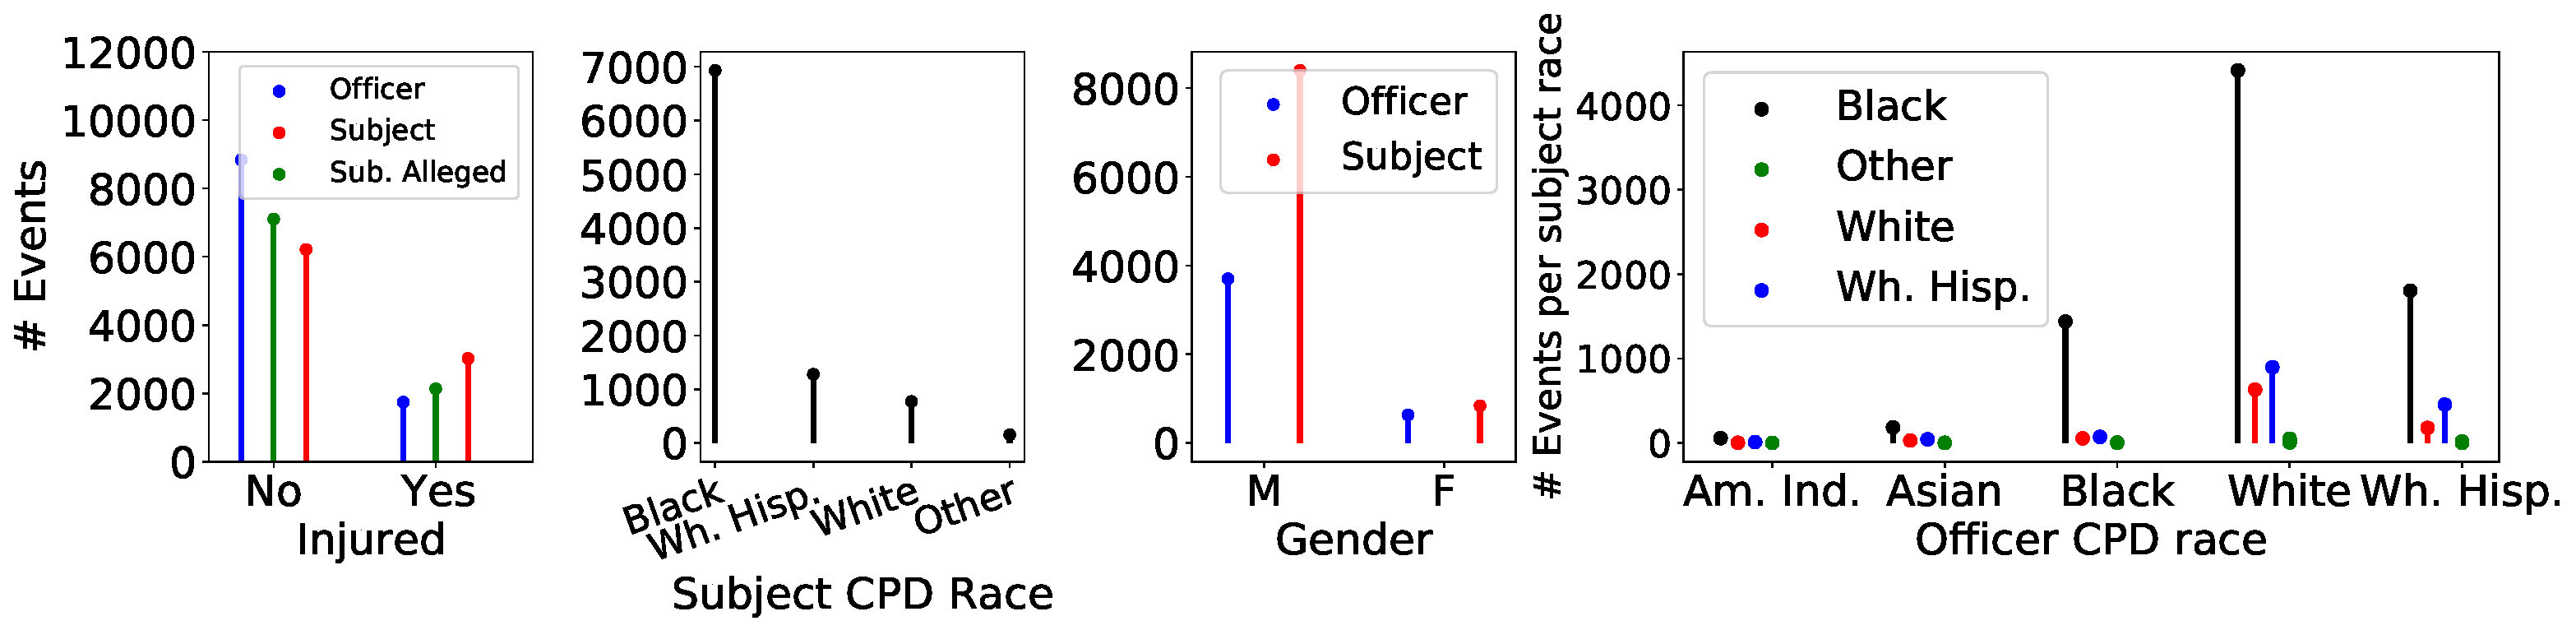
\includegraphics[width=\textwidth]{figs/trr_stats} 
	\caption{Additional statistics for TRRs.} \label{fig:trrs_stats1}
\end{figure}

%\begin{figure}[h] 
%	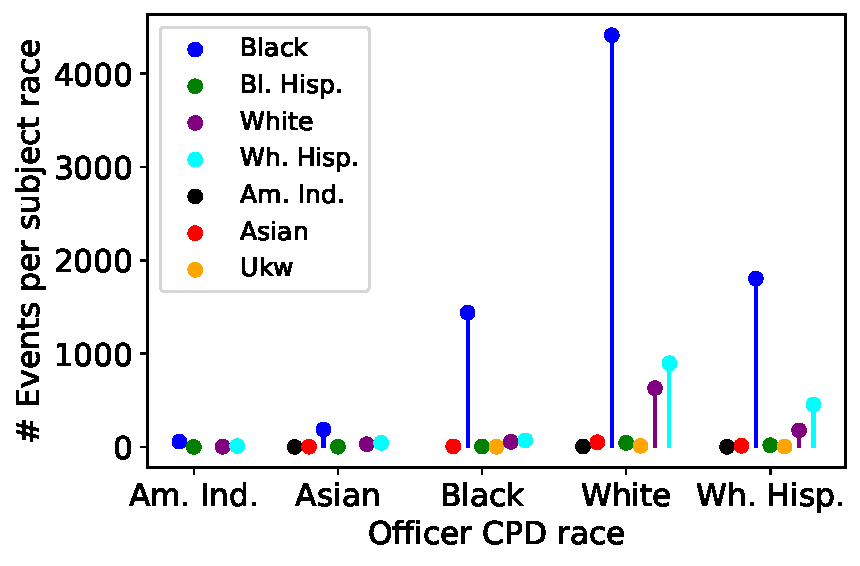
\includegraphics[width=\textwidth]{figs/trr_stats_race_race} 
%	\caption{Temporal data for TRRs.} \label{fig:trrs_stats2}
%\end{figure}

We also report temporal information about the TRRs in \Cref{fig:trrs_times}. TRRs tend to be filed more frequently at night, in the weekends, and during warmer months. Moreover, 2010, 2011 and 2012 are the years in which the highest number of TRRs have been filed. We also report in \Cref{fig:trrs_stats1} additional information about TRRs: in most cases, neither the officers nor the subjects involved get injured, although civilians get injured at a much higher rate (left subplot), and officers tend to fire first. 
\paragraph{Salary.} todo

\begin{figure}[h] 
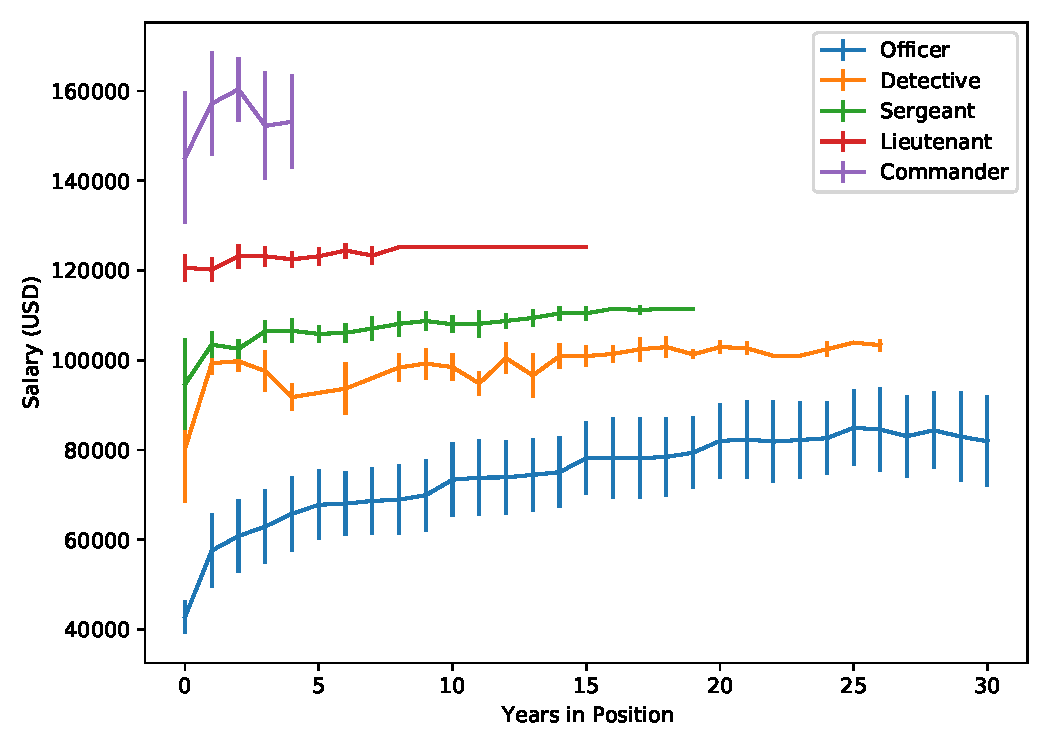
\includegraphics[width=\textwidth]{figs/salary} 
\caption{Historical data from the CPD. Salary versus experience in each
position, years x axis, salary (USD) y axis, for a few of the most common
positions. Lines are means, bars indicate 1 std dev above and below.} \label{fig:salary}
\end{figure}

\begin{figure}[h] 
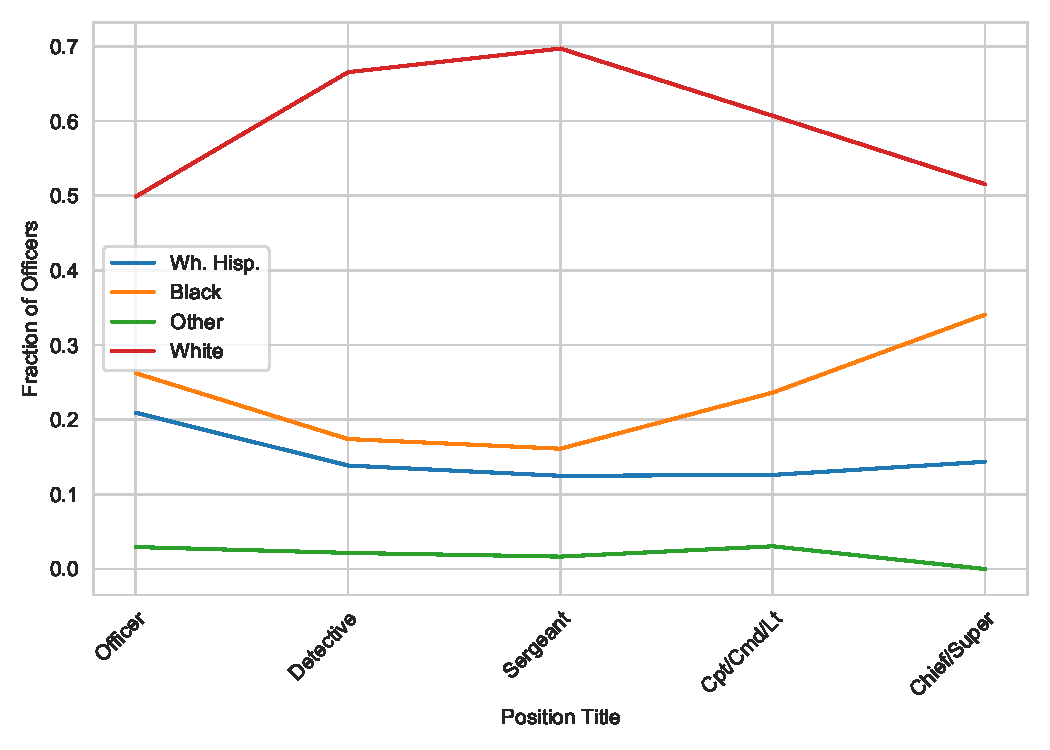
\includegraphics[width=\textwidth]{figs/position_race} 
\caption{Historical data from the CPD. Fraction of officers in representative positions 
per race category.} \label{fig:salary}
\end{figure}

\begin{figure}[h] 
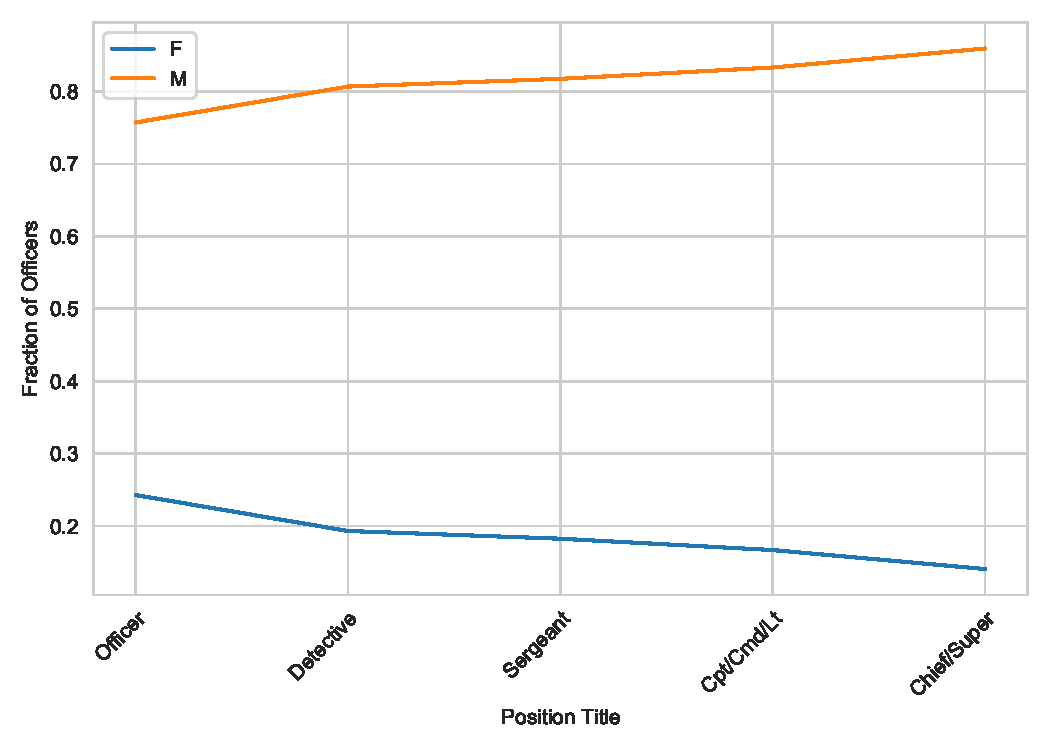
\includegraphics[width=\textwidth]{figs/position_gender} 
\caption{Historical data from the CPD. Fraction of officers in representative positions 
per gender category.} \label{fig:salary}
\end{figure}

\paragraph{Awards.}

\begin{figure}[h] 
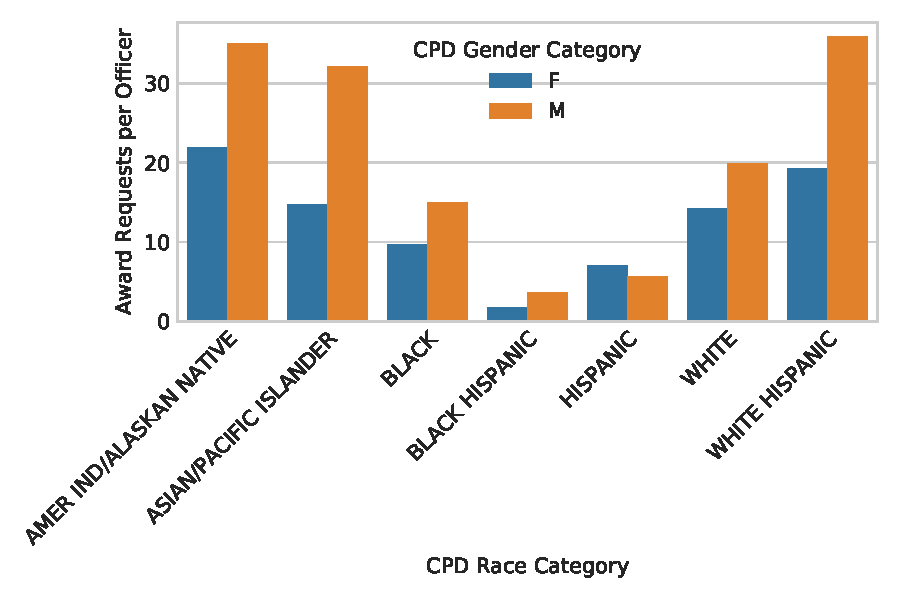
\includegraphics[width=\textwidth]{figs/awards} 
\caption{Historical data from the CPD. Awards per officer vs race for the two cpd gender categories.} \label{fig:awards}
\end{figure}




% !TEX root = ../main.tex
\section{Discussion} \label{sec:discussion}

\subsection{Intended Uses}
Uses for this dataset are varied and rich. For example, researchers could
use the data in a wide variety of predictive tasks, such as
predicting officer misconduct, resignation, and shooting as a function
of their underlying demographic data or complaints filed against them. Past work has engaged
in this type of analysis on both the raw data underlying the present
work, as well as confidential internal police department data \cite{Helsby18,Rozema19}.
This dataset can also be used to study social networks (both in the context of policing and more generally). 
In particular, we can use data in \texttt{complaints\_officers.csv} to construct an
undirected graph $\mathcal{G} = \{\mathcal{V}, \mathcal{E}\}$ in which
$\mathcal{V}$ is the set of nodes---officers appearing in at least one
complaint, and $\mathcal{E}$ the set of edges---where an edge is present
whenever two officers appear on the same complaint. Moreover, we can link the
complaints to the \texttt{tactical\_response\_reports.csv} file to consider
also the subgraph of officers who filed a TRR. We report summary statistics
for the corresponding graphs in \Cref{tab:stats_graphs}, with additional related visualizations
in \cref{sec:additional_figs}.
These networks are of interest in and of
themselves, but can also be used to investigate the dynamic patterns of officer
wrongdoing along such police networks \cite{Roithmayr16}. Existing research has used the complaint
data to identify such patterns and to investigate whether pairs of officers
connected on a network are more likely to have been accused of misconduct \cite{Ouellet19}.
Finally, this dataset could be used to track the effects of new disciplinary
practices, new training techniques, and new oversight on complaints and use of
force. A working paper explores, for example, whether civilians filed fewer
complaints about officers' force in the wake of the Department of Justice
investigation of the Chicago Police Department \cite{Travers20}. 


\begin{table}[t!]
\caption{Summary statistics for the complaints network graph, and the subgraph
of officers in TRRs. All complaints and TRRs filed between 
2004-01-01 and 2015-12-01 are considered in the network construction.
Here LCC is the largest connected component, and Is.~nodes is 
the number of isolated nodes. 
}\label{tab:network}
\begin{tabular}{c|c|c|c|c|c|c|c|}
\cline{2-8}
                                                & $|\mathcal{G}|$ & $|\mathcal{E}|$ & \textit{Avg. degree} & \textit{Triangles} & \textit{Max clique} & \textit{LCC} & \textit{\# Is. nodes} \\ \hline
\multicolumn{1}{|c|}{\textit{\textbf{All}}}     & $14{,}372$      & $106{,}701$     & $14.85$              & $361{,}878$        & $64$                & $13{,}950$   & $0$                   \\ \hline
\multicolumn{1}{|c|}{\textit{\textbf{In TRRs}}} & $4{,}105$       & $22{,}064$      & $10.75$              & $44{,}786$         & $28$                & $3{,}822$    & $225$                 \\ \hline
\end{tabular} \label{tab:stats_graphs}
\end{table}

\subsection{Ethical Considerations}
Recent work on algorithmic fairness focuses on the potential for racially
biased data to produce racially biased results
\cite{veale2018fairness,sloane2019ai,d2020fairness}.  This research suggests
that race shapes data collection in criminal justice, in at least two ways that
are likely to affect data collection on black officers. First, beginning back
in the 1960s, black officers are more likely to be assigned to black
neighborhoods and/or to neighborhoods where police interaction is more
pervasive \cite{Kuykendall80}. Given an increased frequency of interaction,
officers assigned to these neighborhoods may be statistically more likely to be
the subject of complaints \cite{Kane06}.  Second, owing to cognitive bias, complainants 
may be more likely to file a complaint against black officers, either alone or in pairs.
\cref{fig:complaints} provides initial quantitative evidence towards that point. This racial
asymmetry in the collection of complaint data may well produce, for example,
racially biased predictions of police misconduct. Relatedly, because our
dataset may be used to explore predictive policing of the police, black
officers may be unfairly and disproportionately identified to be at higher risk
of misconduct \cite{veale2018fairness,sloane2019ai,d2020fairness,Wood19}. 

\subsection{Limitations and Future Work}
Using civilian and administrator complaint data to study actual (not merely
perceived) police misconduct inevitably faces significant questions about
validity. At least one study has found that because of flaws in police record
keeping and categorization, the practice of using complaints to measure police
behavior is unreliable \cite{Hickman16}. Even so, other research finds a strong
correlation between civilian-filed complaints against officers and internal
complaints against the same officers filed by other officers or supervisors
\cite{Lersch00}. Whatever the truth of the matter, the dataset could be
strengthened by adding more objective measures of misconduct, for example, data
on individual officer misconduct from oversight agencies.

Use of this dataset for network research faces a particular set of limitations.
To wit, researchers who use complaint data to generate social networks must
acknowledge that the co-listing of two officers on a complaint is an
 incomplete proxy for a professional network relationship or
exposure to another officer's misconduct. Data on partner assignment and
dispatches would more accurately reflect officer relationships and their
exposure to misconduct. 

In general, future work should focus on integrating into this dataset as many
objective sources of data on individual officers as possible. Objective data
could include information about adverse incident histories, officer discipline
histories, counseling interventions, domestic violence incidents, weapons
violations, sustained complaints, and lawsuit settlements. Additional information
about officer activities could include partner assignments, dispatch
information, arrest and stop information, unit leadership, and unit disciplinary history. 


\end{document}
